%-*-latex-*-
\sectionthree{The birthday paradox}
\begin{python0}
from solutions import *; clear()
\end{python0}

How many people do you need in order to have at least a pair with
the same birthday?
There are about 365.25 days in a day.
So you would think that you need maybe about half.
Of course the pigeonhole guarantees there will be such a pair if
you have 366 people.

But surprisingly, you actually need a very small group of randomly
chosen people in order to have a good chance (i.e., probability of $> 0.5$)
that at least one pair
has a common birthday.

Since I'm trying to prove that a very small number is enough,
let's round up and say that there are 366 days in a year.

It's easier to ask the opposite question first.
Let $n$ be the number of people you have chosen.
What is the probability that there is \textit{no} two with the same
birthday?

That sounds kind of difficult.
So let's make things concrete,
What if $n = 1$? 
Well ... there's no way for a pair to have the same birthday!
Because there's only one person!
Duh!

OK.
What if there are two?
In other words, what if $n = 2$?
Suppose the birthday of the first person is known.
Then in order for the second person not to have the same birthday
as the first, the second person has a \lq\lq choice'' of birthday
among $366 - 1$ days out of 366 days.
So in this case, the probability is
\[
\frac{366 - 1}{366}
\]

Now what if $n = 3$?
Suppose there are 3 people.
After the first person has announced his/her birthday,
then the probability that the second person has a different birthday as
the first must be 
\[
\frac{366 - 1}{366}
\]
After that, since two birthdays are taken, the probability for the third
person to have a birthday different from the first two must be 
\[
\frac{366 - 2}{366}
\]
Altogether, the probability that among 3 randomly chosen people not to have
the same birthday must be 
\[
\frac{366 - 1}{366} \cdot 
\frac{366 - 2}{366}
\]

In general, you see quickly that if you have $n$ people, the probability
that they all have different birthdays must be 
\[
\frac{366 - 1}{366} \cdot 
\frac{366 - 2}{366} \cdot \cdots \cdot
\frac{366 - (n - 1)}{366}
\]
Of course the probability of have at least a pair with the same
birthday is then
\[
1 - \frac{366 - 1}{366} \cdot 
\frac{366 - 2}{366} \cdot \cdots \cdot
\frac{366 - (n - 1)}{366}
\]

Now I'm interested in knowing when there will be
at least two with the same birthday.
Probabilistically speaking,
that means I want the probability is greater than 0.5.
So I want to find $n$ such that
\[
1 - \frac{366 - 1}{366} \cdot 
\frac{366 - 2}{366} \cdot \cdots \cdot
\frac{366 - (n - 1)}{366} > 0.5
\]
We can find $n$ by running the following program:
\begin{console}[fontsize=\small]
def f(i): 
    return (366 - i) / 366.0

def prob(n):
    p = 1
    for i in range(1, n):
        p *= f(i)
    return 1 - p

for n in range(1, 40):
    print(n, prob(n))
\end{console}
Here's the output:
\begin{Verbatim}[frame=single, commandchars=\\\{\}, fontsize=\small]
1 0
2 0.00273224043716
3 0.00818179103586
4 0.0163114484864
5 0.0270621430384
6 0.0403536438166
7 0.056085551295
8 0.0741385598768
9 0.0943759684041
10 0.116645411804
11 0.140780783066
12 0.166604311444
13 0.193928760249
14 0.222559705923
15 0.252297859249
16 0.282941389607
17 0.314288214105
18 0.34613821509
19 0.378295352052
20 0.410569637055
21 0.442778946506
22 0.474750646296
23 0.506323011819
24 0.537346429109
25 0.567684368184
26 0.597214124456
27 0.625827328729
28 0.653430230708
29 0.679943764971
30 0.705303412009
31 0.729458870041
32 0.752373555912
33 0.774023955395
34 0.794398844663
35 0.813498405541
36 0.83133325747
37 0.847923428867
38 0.863297289883
39 0.877490467436
\end{Verbatim}
Looks like we just need 23, which is surprising small!

To verify this, just get a group of 23 people in a room and ask for their
birthdays then there's a strong likelihood that there are two with the same
birthdays.

It's troublesome to get 23 people together.
So let's write a simple program to pick 23 numbers from 1 to 366
and see if there are two with the same value.
\begin{Verbatim}[frame=single, commandchars=\\\{\}, fontsize=\small]
import random; random.seed()
xs = [random.randrange(1, 367) for _ in range(23)]
xs.sort()
print(xs)
\end{Verbatim}
Here's the output running the above several times.
I've done it 7 times.
Go ahead and count the number of times where there is a repeat
birthday:
\begin{Verbatim}[frame=single, commandchars=\\\{\}, fontsize=\small]
[28, 57, 92, 101, 114, 134, 138, 174, 176, 179, 202, 208, 
218, 231, 239, 241, 251, 253, 283, 286, 294, 317, 325]
[19, 40, 50, 53, 64, 74, 129, 140, 146, 161, 169, 179, 
193, 194, 221, 231, 249, 269, 271, 293, 321, 350, 357]
[14, 36, 43, 55, 83, 124, \underline{133, 133}, 138, 155, 256, 263, 
267, 274, 283, 296, 307, 315, 325, 338, 348, 349, 355]
[4, 41, 44, 80, 119, 124, 136, 139, 140, 163, 183, 212, 
215, 216, 217, 228, 235, 248, 256, 263, 271, 281, 350]
[25, 28, 67, 91, 120, 146, \underline{152, 152}, 196, 206, 222, \underline{223,} 
\underline{223}, 234, 240, 242, 248, 253, 288, 289, 314, 320, 352]
[20, 21, 55, 76, 91, 102, 104, 119, 144, 152, 173, 200, 
204, 206, 214, 222, 230, \underline{249, 249}, 326, 334, 354, 360]
[24, 30, 35, 50, 62, 66, 77, 78, \underline{91, 91}, 121, 150, 153, 
183, 184, \underline{211, 211}, 220, 235, 262, 344, 347, 351]
\end{Verbatim}
Now I'm going to do this 10000 times:
\begin{Verbatim}[frame=single, commandchars=\\\{\}, fontsize=\small]
def repeat(xs):
    for i in range(22):
        if xs[i] == xs[i + 1]:
            return True
    return False

import random; random.seed()
count = 0
for i in range(10000):
    xs = [random.randrange(1, 367) for _ in range(23)]
    xs.sort()
    if repeat(xs): 
        count += 1

print(count)
\end{Verbatim}
Here's my output:
\begin{Verbatim}[frame=single, commandchars=\\\{\}, fontsize=\small]
5103
\end{Verbatim}
So 5103 out of 10000 simulations have a repeat birthday.
When I ran the experiment with 100000 simulations, the number is 
\begin{Verbatim}[frame=single, commandchars=\\\{\}, fontsize=\small]
50519
\end{Verbatim}
In all cases, more than half of the cases of randomly generated
23 birthdays has at least two with the same birthday.

Instead of using a program, let's look at the above expression again:
\[
1 - \frac{366 - 1}{366} \cdot 
\frac{366 - 2}{366} \cdot \cdots \cdot
\frac{366 - (n - 1)}{366} > 0.5
\]
This is
\[
1 - 
\left( 1 - \frac{1}{366} \right)  
\left( 1 - \frac{2}{366} \right)  
\cdots 
\left( 1 - \frac{n - 1}{366} \right)
> 0.5  
\]

We want to find the smallest $n$ satisfying the above.
You can tell that this is not one of the standard equations
from your math classes.
So let me solve this inequality using a program.
(An approximation using math is below.)
Here's the program:
\begin{python}
s = r'''
n = 2
while 1:
    p = 1
    for i in range(1, n):
        p *= (1 - i / 366.0)
    print(n, 1 - p)
    if 1 - p > 0.5:
         break
    n += 1
'''.strip()
f = open('a15245236.py', 'w')
f.write(s)
f.close()
from latextool_basic import *
print(r'{\small %s}' % console(s))
print("and the output")
print(r'{\small %s}' % shell('python a15245236.py'))
\end{python}
\begin{center}
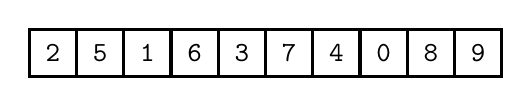
\begin{tikzpicture}

\draw (0.3, -0.3)
  node[draw, line width=0.04cm, , color=black,
       rounded corners=0cm, inner sep=0cm] {

\begin{minipage}[t][0.6cm]{0.6cm}
\mbox{}

\end{minipage}

};\draw (0.3, -0.3) node[color=black] {{\texttt{2}}};
\draw (0.8999999999999999, -0.3)
  node[draw, line width=0.04cm, , color=black,
       rounded corners=0cm, inner sep=0cm] {

\begin{minipage}[t][0.6cm]{0.6cm}
\mbox{}

\end{minipage}

};\draw (0.8999999999999999, -0.3) node[color=black] {{\texttt{5}}};
\draw (1.5, -0.3)
  node[draw, line width=0.04cm, , color=black,
       rounded corners=0cm, inner sep=0cm] {

\begin{minipage}[t][0.6cm]{0.6cm}
\mbox{}

\end{minipage}

};\draw (1.5, -0.3) node[color=black] {{\texttt{1}}};
\draw (2.0999999999999996, -0.3)
  node[draw, line width=0.04cm, , color=black,
       rounded corners=0cm, inner sep=0cm] {

\begin{minipage}[t][0.6cm]{0.6cm}
\mbox{}

\end{minipage}

};\draw (2.0999999999999996, -0.3) node[color=black] {{\texttt{6}}};
\draw (2.7, -0.3)
  node[draw, line width=0.04cm, , color=black,
       rounded corners=0cm, inner sep=0cm] {

\begin{minipage}[t][0.6cm]{0.6cm}
\mbox{}

\end{minipage}

};\draw (2.7, -0.3) node[color=black] {{\texttt{3}}};
\draw (3.3, -0.3)
  node[draw, line width=0.04cm, , color=black,
       rounded corners=0cm, inner sep=0cm] {

\begin{minipage}[t][0.6cm]{0.6cm}
\mbox{}

\end{minipage}

};\draw (3.3, -0.3) node[color=black] {{\texttt{7}}};
\draw (3.9, -0.3)
  node[draw, line width=0.04cm, , color=black,
       rounded corners=0cm, inner sep=0cm] {

\begin{minipage}[t][0.6cm]{0.6cm}
\mbox{}

\end{minipage}

};\draw (3.9, -0.3) node[color=black] {{\texttt{4}}};
\draw (4.5, -0.3)
  node[draw, line width=0.04cm, , color=black,
       rounded corners=0cm, inner sep=0cm] {

\begin{minipage}[t][0.6cm]{0.6cm}
\mbox{}

\end{minipage}

};\draw (4.5, -0.3) node[color=black] {{\texttt{0}}};
\draw (5.1, -0.3)
  node[draw, line width=0.04cm, , color=black,
       rounded corners=0cm, inner sep=0cm] {

\begin{minipage}[t][0.6cm]{0.6cm}
\mbox{}

\end{minipage}

};\draw (5.1, -0.3) node[color=black] {{\texttt{8}}};
\draw (5.699999999999999, -0.3)
  node[draw, line width=0.04cm, , color=black,
       rounded corners=0cm, inner sep=0cm] {

\begin{minipage}[t][0.6cm]{0.6cm}
\mbox{}

\end{minipage}

};\draw (5.699999999999999, -0.3) node[color=black] {{\texttt{9}}};
\end{tikzpicture}

\end{center}


  
Now let's derive that using math (and a calculator).
Note that
\begin{align*}
\left( 1 - \frac{1}{366} \right)  
\left( 1 - \frac{2}{366} \right)  
\cdots 
\left( 1 - \frac{n - 1}{366} \right)  
&\leq e^{-1/366} e^{-2/366} \cdots e^{-(n - 1)/366} \\
&= e^{-(1 + 2 + \cdots + (n - 1))/366} \\
&= e^{-\frac{(n - 1)n}{2}/366} 
\end{align*}
I'm using the inequality
\[
1 + x \leq e^x
\]
which comes from
\[
1 + x + \frac{1}{2!}x^2 + \frac{1}{3!}x^3 + \cdots = e^x
\]
if you recall the Maclaurin/Taylor series for $e^x$.
Or you can derive this by proving $e^x - 1 - x \geq 0$
(standard Calc 1 type problem: show the left-hand side is $ \geq 0$
when $x = 0$ and the slope is $> 0$ for $x > 0$.)

Therefore the above inequality becomes
\[
1 - 
\left( 1 - \frac{1}{366} \right)  
\left( 1 - \frac{2}{366} \right)  
\cdots 
\left( 1 - \frac{n}{366} \right)
\geq 1 - e^{-\frac{(n-1)n}{2}/366}
\]
In that case for an $n$ such that
$1 - \left( 1 - \frac{1}{366} \right)  
\left( 1 - \frac{2}{366} \right)  
\cdots 
\left( 1 - \frac{n - 1}{366} \right)$
is approximately $0.5$,
we have
\[
0.5 \approx 1 - e^{-\frac{(n-1)n}{2}/366}
\]
which gives us
\[
e^{-\frac{(n-1)n}{2}/366} \approx 0.5
\]
Taking natural logs,
\[
(n-1)n \approx (-\ln 0.5) \cdot 738
\]
and therefore
\[
n^2 - n + \ln 0.5 \cdot 738 \approx 0
\]
Solving the quadratic we get
\[
n \approx \frac{1 + \sqrt{1 - 4 \ln 0.5 \cdot 738}}{2} = 23.1228\ldots
\]
(of course taking the positive root).

If instead of 366 days in a year,
if there are $N$ days in a year (say we're on a different planet),
then the minimum value of $n$ to reach about 0.5 is given by
\[
n \approx 
\frac{1 + \sqrt{1 - 4 \ln 0.5 \cdot (2N)}}{2} 
=\frac{1 + \sqrt{1 - 8N \ln 0.5}}{2} 
\]
taking the positive root of the quadratic equation.

%-*-latex-*-

\begin{ex} 
  \label{ex:prob-00}
  \tinysidebar{\debug{exercises/{disc-prob-28/question.tex}}}

  \solutionlink{sol:prob-00}
  \qed
\end{ex} 
\begin{python0}
from solutions import *
add(label="ex:prob-00",
    srcfilename='exercises/discrete-probability/prob-00/answer.tex') 
\end{python0}

%-*-latex-*-

\begin{ex} 
  \label{ex:prob-00}
  \tinysidebar{\debug{exercises/{disc-prob-28/question.tex}}}

  \solutionlink{sol:prob-00}
  \qed
\end{ex} 
\begin{python0}
from solutions import *
add(label="ex:prob-00",
    srcfilename='exercises/discrete-probability/prob-00/answer.tex') 
\end{python0}

%-*-latex-*-

\begin{ex} 
  \label{ex:prob-00}
  \tinysidebar{\debug{exercises/{disc-prob-28/question.tex}}}

  \solutionlink{sol:prob-00}
  \qed
\end{ex} 
\begin{python0}
from solutions import *
add(label="ex:prob-00",
    srcfilename='exercises/discrete-probability/prob-00/answer.tex') 
\end{python0}


The birthday paradox is equivalent to the following
question:
Let there be $n$ people.
They all have been randomly given a value $v$ from
a set of size $k$ in the following way:
Your $k$ value are written on a piece of paper,
you close your eyes and point your finger, and that value is given to a person.
You repeat until every person in your group of $n$ people has been assigned a value.
What is the probability that at least two have been given the same value?


The birthday paradox is important in
cryptography and hash tables because of hash collisions.

In the case of the hash table data structure,
if you choose an array of linked list as implementation,
collisions imply a longer linked list for each hash value of the keys
and the worse runtime is determined by the length of the longest
linked list.

In the case of digital signatures,
assuming you are using the RSA version with pair of keys $(k_0, k_1)$,
to sign a message $m$, Alice would compute $m' = D(h(m), k_1)$
which would be the digital signature.
Here $h$ is the hash function and
$(E(k_0, \bullet), D(k_1, \bullet))$ are the encryption-decryption pair of functions
for Alice's keys $(k_0, k_1)$ where $k_0$ public and $k_1$ is private.
Alice sends $(m, m', h(m))$ to Bob.
Bob can read the message $m$,
but Bob also want to be certain that $m$ is from Alice.
So Bob computes
\[
  E(k_0, m')
\]
If $m' = D(k_1, h(m))$, i.e., it's really created by Alice (assuming no one else has $k_1$,
only Alice can create $m'$), then
$E(k_0, m')$ must be $h(m)$.

Suppose Eve intercepts $(m, m', h(m))$.
She then creates
another message $m^*$ such that
$h(m^*) = h(m)$
and then sends $(m^*, m', h(m))$ to Bob.
Bob computes
\[
  E(k_0, m') = h(m) = h(m^*)
\]
and thinks that $m^*$ is signed by Alice.
Bob is counting on the fact that it's difficult to find another
$m^*$ such that $h(m^*) = h(m)$.
(The above is a textbook example of digital signatures.
In real life, there are a few more things to do.
Furthermore the
message $m$ itself is usually
encrypted.)

\begin{comment}
BDAY paradox with random variables]

Recall that for the probability of having 2 people among $n$
to have the same birthday to be $> 1/2$, we need $n \geq 23$.

There's an analogus method that uses random variables.

Assume there are $n$ people in the room.
Let $X_{ij}$ be the indicator rv that the $i$--th and $j$--th persons
have the same birth.
Therefore 
\[
E \left[ \sum_{i=1}^{n} \sum_{j=i+1}^{n} X_{ij} \right]
\]
is the number of people in the room whose birthday falls on the
same day as someone else in the room, without double-counting.
(Without double-counting means is John's birthday equals Tom,
then we count John,Tom as a matching pair \textit{once}.)

In more details, let $S = \{1, ..., 366\}^n$, i.e., the
set of $n$--tuples where each value of a tuple is taken from the set
$\{1, ..., 366\}$.
I'm assuming that there are 366 days per year.
Let $p : S \rightarrow \R$ be the uniform pdf on $S$, i.e.,
$p$ is the product of $n$ uniform pdfs on $\{1, ..., 366\}$.
Define $X : S \rightarrow \R$ as follows: let
$s = (s_1, ..., s_{366}) \in S$. Then
\[
X(s) = \text{number of $s_i$'s that equals some $s_j$
where $i < j$}
\]
We can also define $X_{ij} : S \rightarrow \R$ such that
for $s = (s_1, ..., s_n) \in S$,
\[
X_{ij}(s) =
\begin{cases}
  1 & \text{if $s_i = s_j$} \\
  0 & \text{otherwise}
\end{cases}
\]
Then
\[
X =
\sum_{i=1}^{n} \sum_{j=i+1}^{n} X_{ij}
\]

Note that
\[
E \left[ X_{ij} \right] = \frac{1}{366}
\]
Why? Because
\[
E \left[ X_{ij} \right] = \sum_{s \in S} X_{ij}(s) p(s)
\]
and the only term that is nonzero is when $X_{ij}(s) = 1$
where $s_i = s_j$
and it's easy to see that in this case
$p(s) = 1/366$: For the case where $s_i = 1 = s_j$, there
are $366^{n-2}$ tuples,
for the case where $s_i = 2 = s_j$, there are
$366^{n-2}$ tuples, etc.
Therefore there are $365^{n-2} \cdot 365 = 365^{n-1}$ tuples
where $s_i = s_j$.
Therefore $p(s) = 365^{n-1}/|S| = 365^{n-1}/365^n = 1/365$.

There's another way to think about the above:
Let
\[
A
=
\{s \mid \text{there is some $i$ such that }
s_i = s_j \text{ for some $j > i$}\}
\]
Now for each $i$,
\[
A_i = \{s \mid s_i = s_j \text{ for some $j > i$}\}
\]
Then
\[
A = \dot{\bigcup}_{i=1}^n A_i
\]
(the union is disjoint).

Hence the number of pairs of people with non-unique birthdays is given by
\[
E \left[
  \sum_{i=1}^{n} \sum_{j=i+1}^{n} X_{ij}
  \right]
  =
  \sum_{i=1}^{n} \sum_{j=i+1}^{n} 
  E \left[X_{ij}\right]
  =
  \binom{n}{2}\frac{1}{366}
\]
Therefore for there to be at least a pair with the same birthdays is the
same as saying
\begin{align*}
     & \binom{n}{2} \frac{1}{366}  \geq 1 \\
\iff & \,\,\,\,\, \frac{n(n-1)}{2} \geq 366 \\
\iff & \,\,\,\,\, n(n-1)           \geq 2 \cdot 366 \\
\iff & \,\,\,\,\, n^2 - n - 2 \cdot 366 \geq 0\\
\end{align*}
The roots of $x^2 - x - 2 \cdot 366$ are
\[
x = \frac{1 \pm \sqrt{1 + 4 \cdot 2 \cdot 366}}{2}
\]
The positive root is approximately $27.56...$.
Therefore if there are at least 28 people, you will have a pair with
the same birthday.
Therfore
\begin{align*}
  E \left[
  \sum_{i=1}^{n} \sum_{j=i+1}^{n} X_{ij}
  \right] \geq 1
\iff & \,\,\,\,\, n^2 - n - 2 \cdot 366 \geq 0\\
\iff & n \geq 28
\end{align*}

Note that
$E \left[
  \sum_{i=1}^{n} \sum_{j=i+1}^{n} X_{ij}
\right] \geq 1$
is not the same as
probability of finding a pair with the same birthday.

??? Consider $X_{23}, X_{34}, X_{24}$.
What is 
Suppose I have a 366 sided die.


Suppose an outcome is $x = (5, 3, 2, 3, 5, 3, 7, 8)$ (person 0 has bday 5, person 1 has bday 3, etc.)
Note that $x[1] = x[3]=3$, $x[1] = x[5]=3, x[3]=x[5]=3$, $x[0]=x[4]=5$.
So $E = 4$ (expected number of collisions) and
$p = 4/C(9,2) = 4 / (9*8/2) = 1/9$ (probability that there is a pair of common bday).

\begin{itemize}

  \li
  Each experiment is 23 rolls of the die.
  Count the experiments you have two common roll out of the 23.
  Divide the count by the number of experiments to get a number that is $> 0.5$.

  If you do 1000 of this experiment, about 500 of them will have no pairs
  and 500 will have a pair (or more).
  That gives an average of 0.5.

  But what if I want to count the number of pairs?
  According to the above, if I use 23 rolls for each experiment, 
  then 500 of them will have no pairs and 500 of them will have a pair (or more).
  If 500 will have exactly pair, then the average number of pairs will be 0.5.
  Which means 23 is too small.
  That's why for the expectation computation, you need 28.

  \li
  Exact experiment is 28 rolls of the die.
  Count the number of pairs common rolls
\end{itemize}
  
Compare the two mathematically:
\[
  p > 0.5
\]
is
\[
1 - 
\left( 1 - \frac{1}{N} \right)  
\left( 1 - \frac{2}{N} \right)  
\cdots 
\left( 1 - \frac{n}{N} \right)
\geq 1 - e^{-\frac{(n-1)n}{2}/366}
> 0.5
\]
is the approximation sharp enough for the above ineq?
The expected value is
\[
E \left[ \sum_{i=1}^{n} \sum_{j=i+1}^{n} X_{ij} \right] = \binom{n}{2} \frac{1}{N}
\]

xxxxx




Let $n$ be the number of people who share the same birthday
and $N$ be the number of days.
Then the expected number of people who share a birthday with someone is
\[
n(1 - (1 - 1/N)^{n-1})
\]
So
\[
n(1 - (1 - 1/N)^{n-1}) \geq 1
\]
The graph shows that this happens with $n \geq 20$ (the value of the
expression is then 1.11823...)
Why is this not 23?

Note the difference:
\begin{tightlist}
  \item If there are 23 people, then the probability that there's a
  pair with the same birthdays is approximately $0.5$
  \item If there are 28 people, then the expected number of pairs
  of same birthdays is $\geq 1$.
\end{tightlist}

They sound the same, but in fact they are different (which is why the
above computation yields two different values or 23 and 28.)

The probability computation tells us that when you have 23 or more people
in a room, it's more likely that there is a pair of people with the same
birthday.
What about the expectation computation?
Let $p(i)$ denotes the probability that there
are exactly $i$ people each of
whom can be paired up with someone else who has the same birthday.
Then the probability that there is at least one pair with the same birthday is
then
\[
\sum_{i=2}^n p(i)
\]
The expectation computated above on the other hand is
\[
\sum_{i=0}^n p(i) \cdot i
\]
(Of course by definition $p(0) = p(1) = 0$. Right?)

Something's not right.
Consider a box with 6 red balls and 4 black balls.
The probability of picking a red is $6/10 > 0.5$.
The expectation of picking a red is $6/10 \cdot 1 + 4/10 \cdot 0 = 6/10$
and not 1.
Or consider the case where the box has $n$ red balls
and 4 black balls.
For the probability of picking a red is $n / (n + 4)$.
For this to be $> 0.5$, $n / (n + 4) > 0.5$
which give $2n > n + 4$ which is $n > 4$.
The expectation of picking a red is
$(n/(n+4)) \cdot 1 + (4/(n+4)) \cdot 0 = n/(n + 4)$.
For this to be $\geq 1$, we get $n/(n + 4) > 1$
which is impossible.




\subsection{From a website}

\url{https://math.stackexchange.com/questions/35791/birthday-problem-expected-number-of-collisions?utm_medium=organic&utm_source=google_rich_qa&utm_campaign=google_rich_qa!}

Let $X$ be the r.v. for number of people with non-unique
birthdays.
In other words if $s = (s_1, s_2, \ldots, s_n) \in S$,
then
\[
X(s)
=
|\{
s_i \mid 1 \leq i \leq n, \,\,\, s_i = s_j
\text{ for some $j \neq i$, $1 \leq j \leq n$}
\}|
\]
Let $X_i$ be
\[
X_i(s)
=
|\{
s_i \mid \,\,\, s_i = s_j
\text{ for some $j \neq i$, $1 \leq j \leq n$}
\}|
\]
Then
\[
X = \sum_{i=1}^n X_i
\]
Note that this does not count the number of \textit{pairs} of people
with same birthdays.
This counts the number of people.
For instance if $n = 2$ and $s = (1, 1)$,
then $X_1(s) = 1$ and $X_2(s) = 1$
since for this selection of people, both have Jan 1 as their birthdays.
This $X$ will give 2 while the $X$ from the previous section gives 1.


From website
\[
E[X] = np
\]
where
\[
p = n(1 - (1 - 1/N)^{n-1})
\]

Note that if we want to have one person with nonunique birthdays,
then we need $X \geq 2$.
So we need to find $n$ such that
\[
E[X] = n(1 - (1 - 1/366)^{n-1})
\]

Here's a program to find the $n$.
\begin{python}
N = 366
for n in range(1, 31):
    print(n, n*(1 - (1 - 1.0/N)**(n-1)))
    print()
\end{python}
This means that $n$ have to be at least roughly 28 or 29 for
$X$ to achieve a value of 2.




\subsection{Comparing the above two methods}

The probability method: Find the smallest $n$ such that
\[
p = 1 -
\left(1 - \frac{1}{366}\right) \cdot 
\left(1 - \frac{2}{366}\right) \cdot
\cdots \cdot
\left(1 - \frac{365}{366}\right) > 0.5
\]
The expectation method: Find the smallest $n$ such that
\[
E[X] =
n
\left(
  1 - \left(1 -\frac{1}{366}\right)^{n-1}
\right)
\geq 2
\]

Average number of pairs with same birthday:


\subsection{Generalizations}



\end{comment}
